\Section{JSARTOOLKIT}
\label{sec:jsartoolkit}

The application of the JSARToolKit library to this project is present in the implementation of a functionality similar to that of the basic sample in the original ARToolKit library. In that sample, the library is used to recognize the markers in the webcam's video stream, and to retrieve the transformation matrices which are used to place 3D models in the same ``place'' (position, orientation and scale). The JSARToolKit library does possess a similar sample in its release bundle, but a lack of documentation or explanation difficulted its use. Other specific tutorials exist among the online community, but these suffer from the same problems of lack of documentation and/or outdated code which is no longer functional.

The first step in this project was setting the system to allow the browser to use the webcam stream in real time. Such preparation is explained in \Cref{sec:setup}. The webcam stream is loaded to a \texttt{video} HTML tag, and in each frame a canvas is redrawn using the stream (the image in this canvas is later analyzed in the search for markers). The second step involved recreating the basic sample by adding the marker recognition to the result of the first step through the analysis of the code in the mentioned faulty tutorials and samples.

The JSARToolKit library uses a raster object which receives a canvas with images to analyze. This raster is then used by a detector which retrieves the information about all the markers present in the scene. The library is quite sensible to light variations and color changes. It is possible for a marker to be present in the image and not be detected (weaker illumination, shadow, or other visual noise). In each frame, the detector is used in the image retrieved from the webcam and each marker is properly identified and added to a structure.

The lack of stability in the detector (it is common for markers to disappear every other frame) is compensated by using an aging process for each marker. When a marker seizes to be detected, instead of immediately removing it from the detected markers list, it is aged across time. Only when that age reaches a certain limit will it be removed.

The second part of the basic sample places a cube on the marker. For this, the Three.js library was used, which allowed to remove much of the complexity intrinsic to the creation of a virtual scene using WebGL.

\begin{figure}[p]
	\begin{center}
		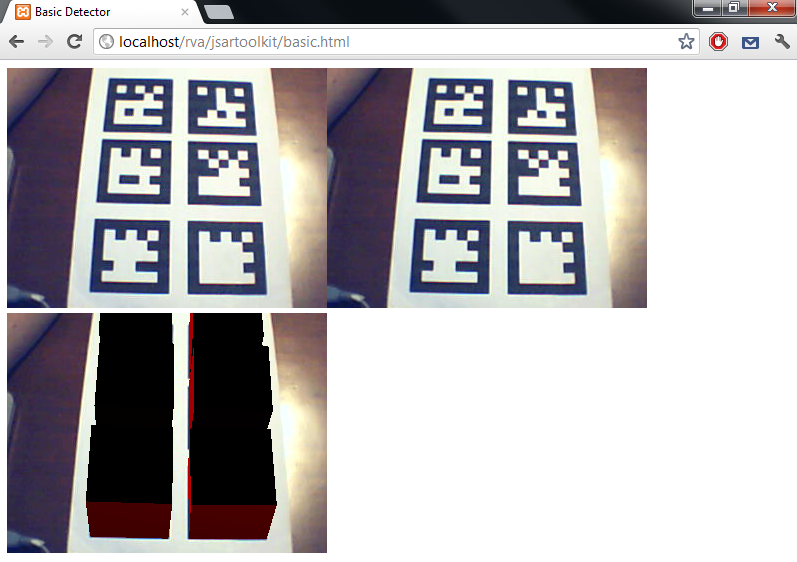
\includegraphics[width=\columnwidth]{report/images/basic.png}
	\end{center}
	\caption[Basic Sample]{Implementation of the basic sample with JSARToolKit. At the top, the \texttt{video} tag showing the webcam stream (left) and the canvas drawing the stream image in each frame (right). In the bottom, the canvas holding the two WebGL 3D scenes: one only with a billboard, showing the video; the other drawing the cubes on top of the markers.}
	\label{fig:basic}
\end{figure}
